\chapter{Distributed Coded Training on the Cloud} \label{ch-2}



\section{Experimental results}
\label{sec:experiments}

In this section, we evaluate the performance of proposed schemes by training multiple neural network models concurrently. We use the AWS Lambda,
% \footnote{https://aws.amazon.com/lambda/}
a fully-managed and cost-efficient serverless cloud computing service. Workers are invoked from the master node using HTTP requests, and task results are received in the HTTP response payload. Appendix~\ref{sec:lambda} provides a detailed discussion of our network setup and cloud resources.

\subsection{Analysis of response time}
\label{subsec:response-time}

Our experiment setup consists of a master node and $n=256$ workers. In Fig.~\ref{fig:4-1}, we demonstrate statistics of response time across $100$ rounds, where each worker calculates gradients for a batch of $16$ MNIST images on a CNN involving three convolutional layers, followed by two fully connected layers.  Fig.~\ref{fig:4-1}(a) shows the response time of each worker at every round. White cells represent stragglers. As discussed in Sec.~\ref{sec:setting}, a worker is deemed straggler when its response time exceeds $(1+\mu)$ times the response time of the fastest worker in the round. For the sake of consistency, we choose $\mu=1$ for all experiments. Nonetheless, such a choice of $\mu$ is by no means critical to observe stragglers. This can be seen in Fig.~\ref{fig:4-1}(c), where the empirical CDF of workers' completion time exhibits a relatively long tail. Fig.~\ref{fig:4-1}(b) plots the number of straggler bursts of different length over this response profile. It can be observed that our response profile does not include nodes that continue to remain stragglers for long duration. This motivates the use of coding across the temporal dimension as proposed in the present work.


\begin{figure}[h]
    \centering
    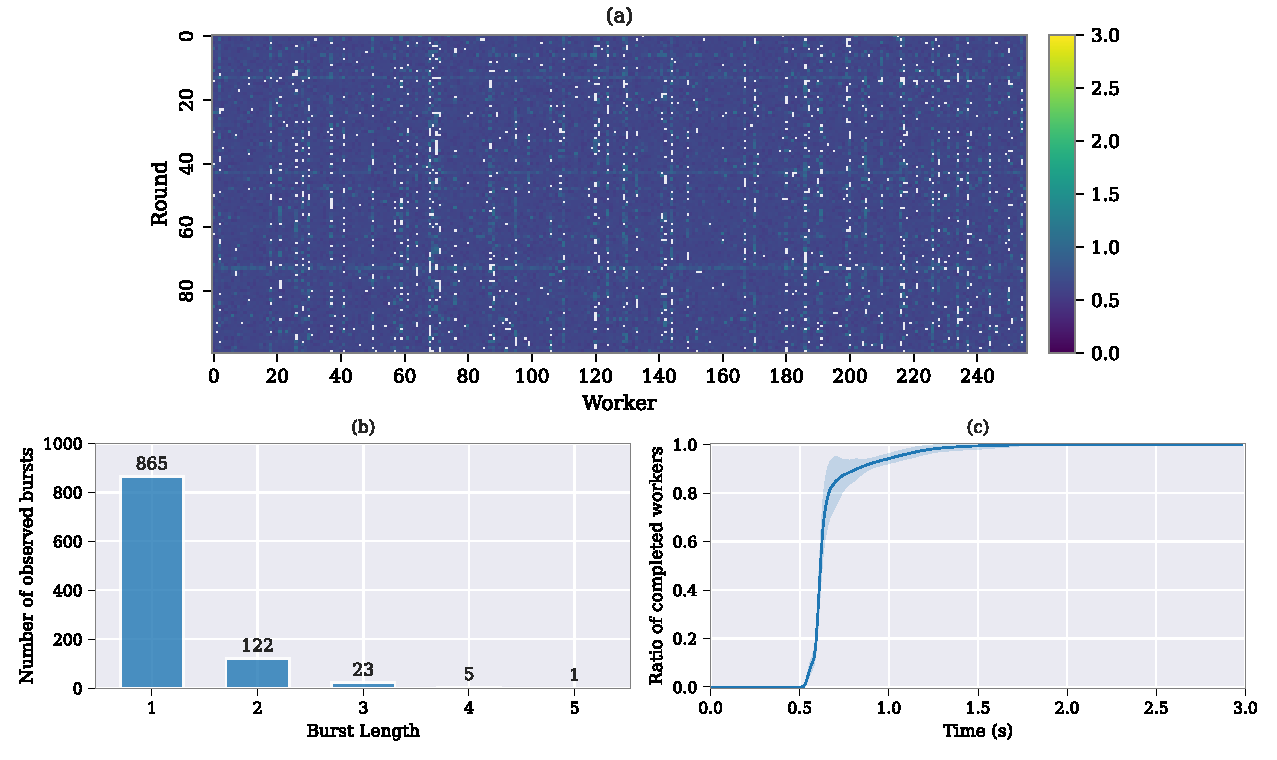
\includegraphics[width=\textwidth]{figures/ch2/fig1.pdf}
    \caption{Statistics of response time for 256 workers across 100 rounds. Each worker calculates gradients of the loss for a batch of 16 MNIST images on a convolutional neural network. (a) Each white cell represents a worker (x-axis) who is a straggler at the corresponding round (y-axis). (b) Histogram of stragglers' burst lengths. (c) Empirical CDF of workers' completion time, averaged over 100 rounds (shades represent standard deviation).}
    \label{fig:4-1}
\end{figure}

\subsection{Comparison of coding schemes}

Using the setup described in Sec.~\ref{subsec:response-time}, we train $M=4$ CNN classifiers for MNIST concurrently following the approach stated in Remark \ref{rem:job_dependency}. In every round, master samples a batch of $4096$ data points and distributes them among the workers. Non-straggling workers compute partial gradients and return task results to the master at the end of each round. After completion of one update, master uploads the updated model parameters to a shared network file system, accessible to the workers.  We use cross entropy as the loss function and ADAM as the optimizer. Moreover, the same dataset and architecture are used for all the models.

In each experiment, we run a total of $J=480$ jobs (120 jobs per classifier) using the three schemes, namely GC, SR-SGC and M-SGC. As a baseline, we also train the classifiers without any coding wherein the master node should wait for all the workers to return their task results. Finally, each experiment is repeated 10 times to report the first and second-order statistics of total run times. Before training the models, we perform some shorter experiments to choose the best-performing parameters for each of the three coding schemes. Specifically, for GC, we perform a grid search over $s$ and select the value corresponding to the shortest run time. We refer readers to Appendix~\ref{sec:param_selection} for the exact procedure of selecting the parameters for SR-SGC and M-SGC schemes.
% \textcolor{blue}{We should at least explain here why $s=15$ for GC was chosen} 

Table \ref{table:4-1} presents the total run time achieved by each coding scheme, along with the selected parameters and resulting normalized loads.
Selection of small values for parameters $B$ and $W$ in our sequential coding schemes matches the empirical evidence in Fig.~\ref{fig:4-1}(b) that isolated short-length-bursts are prevalent. It is interesting to note that the effective value of parameter $s$ in SR-SGC ($s=12$) turns out to be close to that of GC ($s=15$).  Fig.~\ref{fig:4-2}(a) plots total number of completed jobs (for all $M=4$ models) across time, and Fig.~\ref{fig:4-2}(b) shows the course of training loss (of the first model out of the $4$ models) as a function of  time, for all coding schemes. 

\vspace{-0.5em}
\begin{table}[h]
\caption{Total run time achieved by different coding schemes} \label{table:4-1}
\vspace{-1em}
\begin{center}
\begin{tabular}{lccl}
\multicolumn{1}{c}{\bf Scheme}  &\multicolumn{1}{c}{\bf Parameters} &\multicolumn{1}{c}{\bf Normalized Load} &\multicolumn{1}{c}{\bf Run Time (s)} 
\\ \hline \\
M-SGC	   	&$B=1, W=2, \lambda=27$	&$0.008$    &$891.37 \pm 43.10 $\\
SR-SGC	   	&$B=2, W=3, \lambda=23 \; \ (s=12)$	&$0.051$    &$994.22 \pm 43.66 $\\
GC	       	&$s=15$	                &$0.062$    &$1064.96 \pm 46.72$ \\
No Coding	&$-$	                &$0.004$    &$1307.79 \pm 61.88$ 
\end{tabular}
\end{center}
\end{table}
\vspace{-1.5em}

\begin{figure}[h]
    \centering
    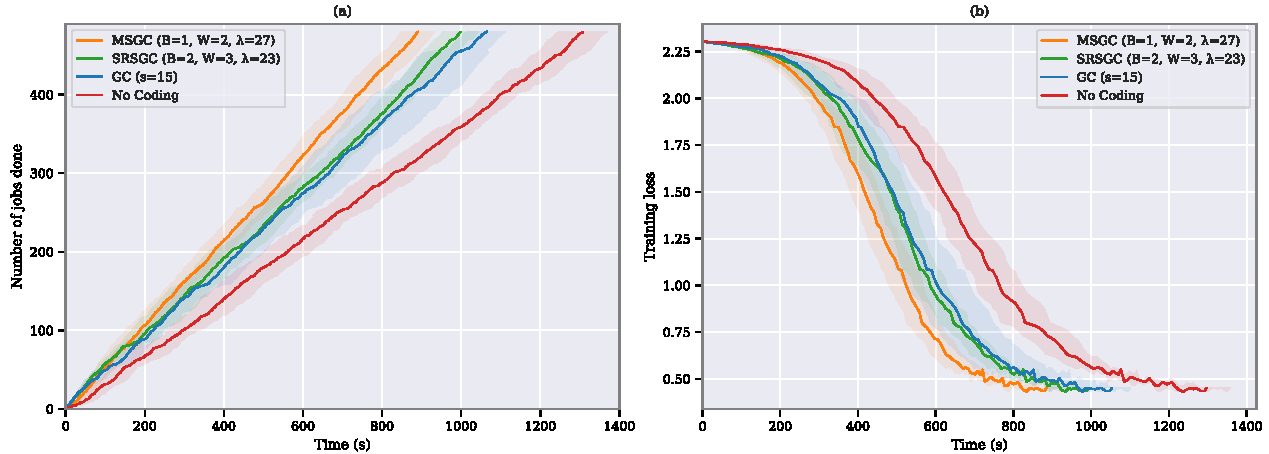
\includegraphics[width=\textwidth]{figures/ch2/fig2.pdf}
    \caption{(a) Number of completed rounds vs. clock time, averaged over 10 independent experiments. (b) Training loss vs. clock time for the first model (out of four concurrently trained models), averaged over 10 independent runs. Shades here represent standard deviation.}
    \label{fig:4-2}
\end{figure}

The first clear observation from Table \ref{table:4-1} is that our proposed M-SGC achieves 16\% lower run time while maintaining smaller normalized load compared to the classical GC scheme. Furthermore, compared to GC, SR-SGC shows slight improvements in total runtime and normalized load simultaneously, demonstrating the potential of incorporating selective repetition into GC. Next, as shown in Fig.~\ref{fig:4-2} and Table \ref{table:4-1}, the existence of stragglers is validated by the fact that any of the coding schemes significantly outperforms the case of not using any coding. This is indeed in line with the empirical observation of Figure \ref{fig:4-1}(c), where the tail of the cumulative distribution of workers' completion time signals the existence of stragglers.





\section{AWS Lambda architecture}\label{sec:lambda}

This section discusses the overall architecture, limitations, and additional details about the setup and usage of the AWS cloud resources used in our experiments (Sec.~\ref{sec:experiments}). 

We use AWS Lambda functions as workers in our distributed training experiments. Each Lambda instance has $2500$ MB of RAM, $1$ vCPU, and supports Python 3.8 runtime environment. A Lambda layer is used to inject external dependencies into the runtime environment (e.g. PyTorch, TorchVision, NumPy etc). Since the size of required external libraries exceeds the 200MB limit of Lambda layers, we zip some libraries in the layer package and unzip them at the time of Lambda instance creation. Note that this will not affect workers' run times as we perform a \textit{warm-up} round before each experiment to ensure that our Lambda instances are initialized and functional. 

Another limitation concerning the use of Lambda functions for training ML models is the total payload size quota of $6$ MB. i.e., the total sum of payload sizes in the HTTP request and response cannot exceed $6$ MB. Note that ideally the master includes current model weights in the HTTP request payload, and receives the task results via the HTTP response payload. This incurs a serious limitation on any reasonably-sized neural network. To overcome this, we need to use a proxy storage service to communicate model weights and task results.

Fortunately, we have two storage options; Amazon S3 (Simple Storage Service) and AWS EFS (Elastic File System). We use the latter, as it will provide higher throughput. EFS is a shared network file system that will be mounted on all Lambda instances at their time of creation. This way, it can be used as a means for communication between the master and workers. In our experiments, we reserve the payload limit for the task result communication, and use EFS to communicate updated model weights to workers, as depicted in Figure \ref{fig:aws} (a). The overall architecture of our cloud resources is shown in Figure \ref{fig:aws} (b). We use AWS Serverless Application Model (SAM) tool to define, manage, and deploy the cloud resources (included in the code submitted as supplementary material).  

\begin{figure}[h]
	\centering
	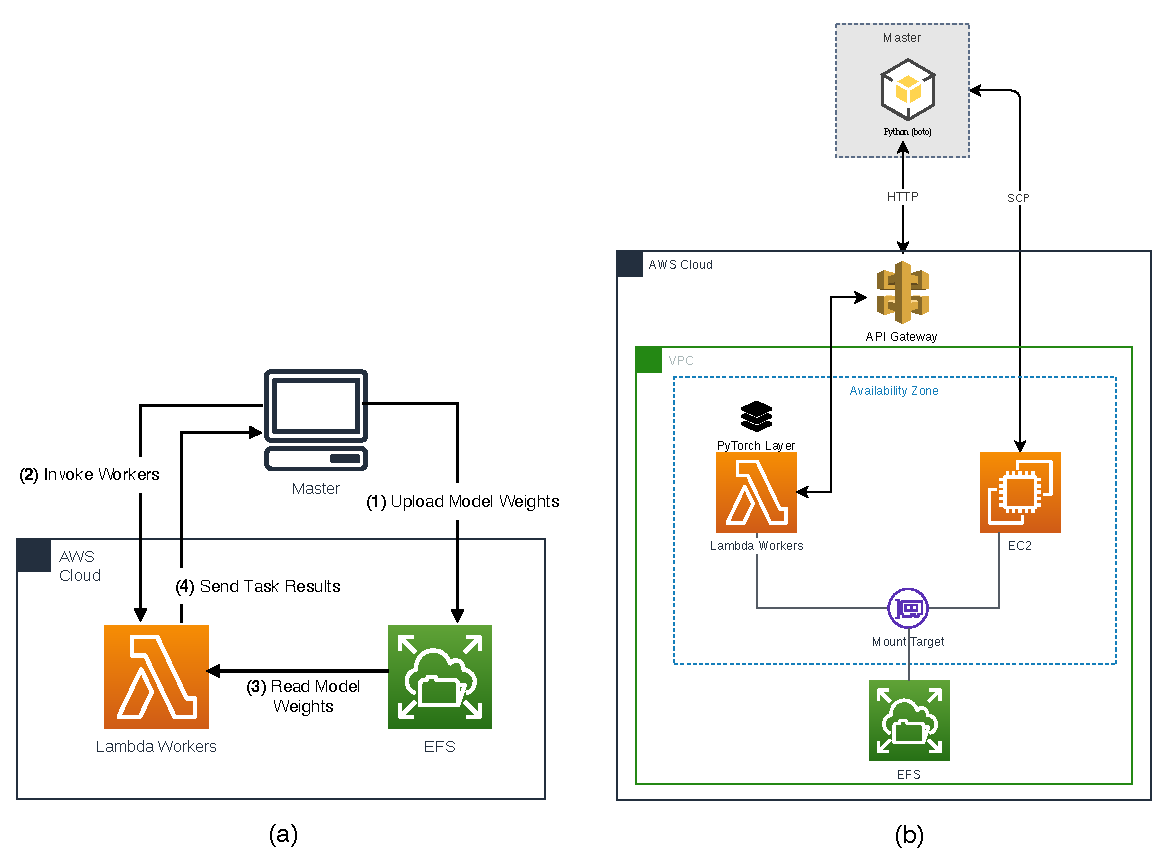
\includegraphics[width=\textwidth]{figures/ch2/aws.pdf}
	\caption{(a) Communication between master and Lambda workers for each round. (b) The overall architecture of AWS cloud resources used.}
	\label{fig:aws}
\end{figure}

\section{Selecting coding scheme parameters}\label{sec:param_selection}

This section discusses the parameter selection method used for our proposed sequential gradient coding schemes, SR-SGC and M-SGC. We begin by noting that the total number of valid parameter combinations for each of these schemes are too large for a grid search to be feasible, as evaluation of each parameter combination requires training models for multiple rounds. Instead, we utilize the observation that increasing the normalized load will linearly increase the average runtime of the workers. Fig.~\ref{fig:base_comp} shows the average runtime of 256 workers across 100 rounds for some values of load $\in [0, 1]$. 

\begin{figure}[h]
	\centering
	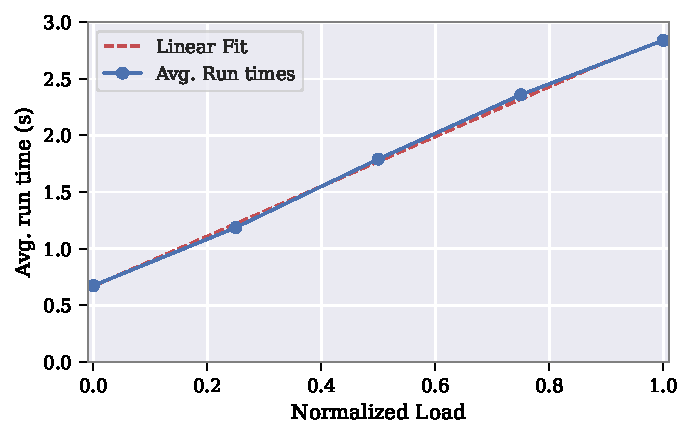
\includegraphics[width=0.45\textwidth]{figures/ch2/5.pdf}
	\caption{Average run time scales linearly with increase in workers' computational load.}
	\label{fig:base_comp}
\end{figure}

We can exploit the observation above to estimate the delay profile corresponding to various coding schemes with variable normalized loads. After estimating the slope of linear fit in Fig.~\ref{fig:base_comp} (let this be $\alpha$), we run our distributed training experiment for $80$ jobs with no coding, and store the observed runtime of workers across rounds (we call this the \textit{reference delay profile}). The normalized worker load in case of no coding will be $1/n$. 
Next, considering a coding scheme with fixed parameters (and therefore a fixed load $l$), we opt to feed this profile to the master node to simulate the run time of workers. However, note that we have to take into account the increase in the workers' run time due to the increase of the load from $1/n$ to $l$. Based on our previous discussion, we can compensate for this increase by adding $(l - 1/n) \alpha$ seconds to our reference delay profile. Using this \textit{translated} delay profile, and based on the assumed coding scheme, the master node will try to resolve stragglers at each round, and if not, it will wait out all the workers, resulting in a simulated total run time for the coding scheme. Fig.~\ref{fig:allparams} shows the result of the above procedure for all valid parameter combinations of SR-SGC and M-SGC. 

\begin{figure}[h]
	\centering
	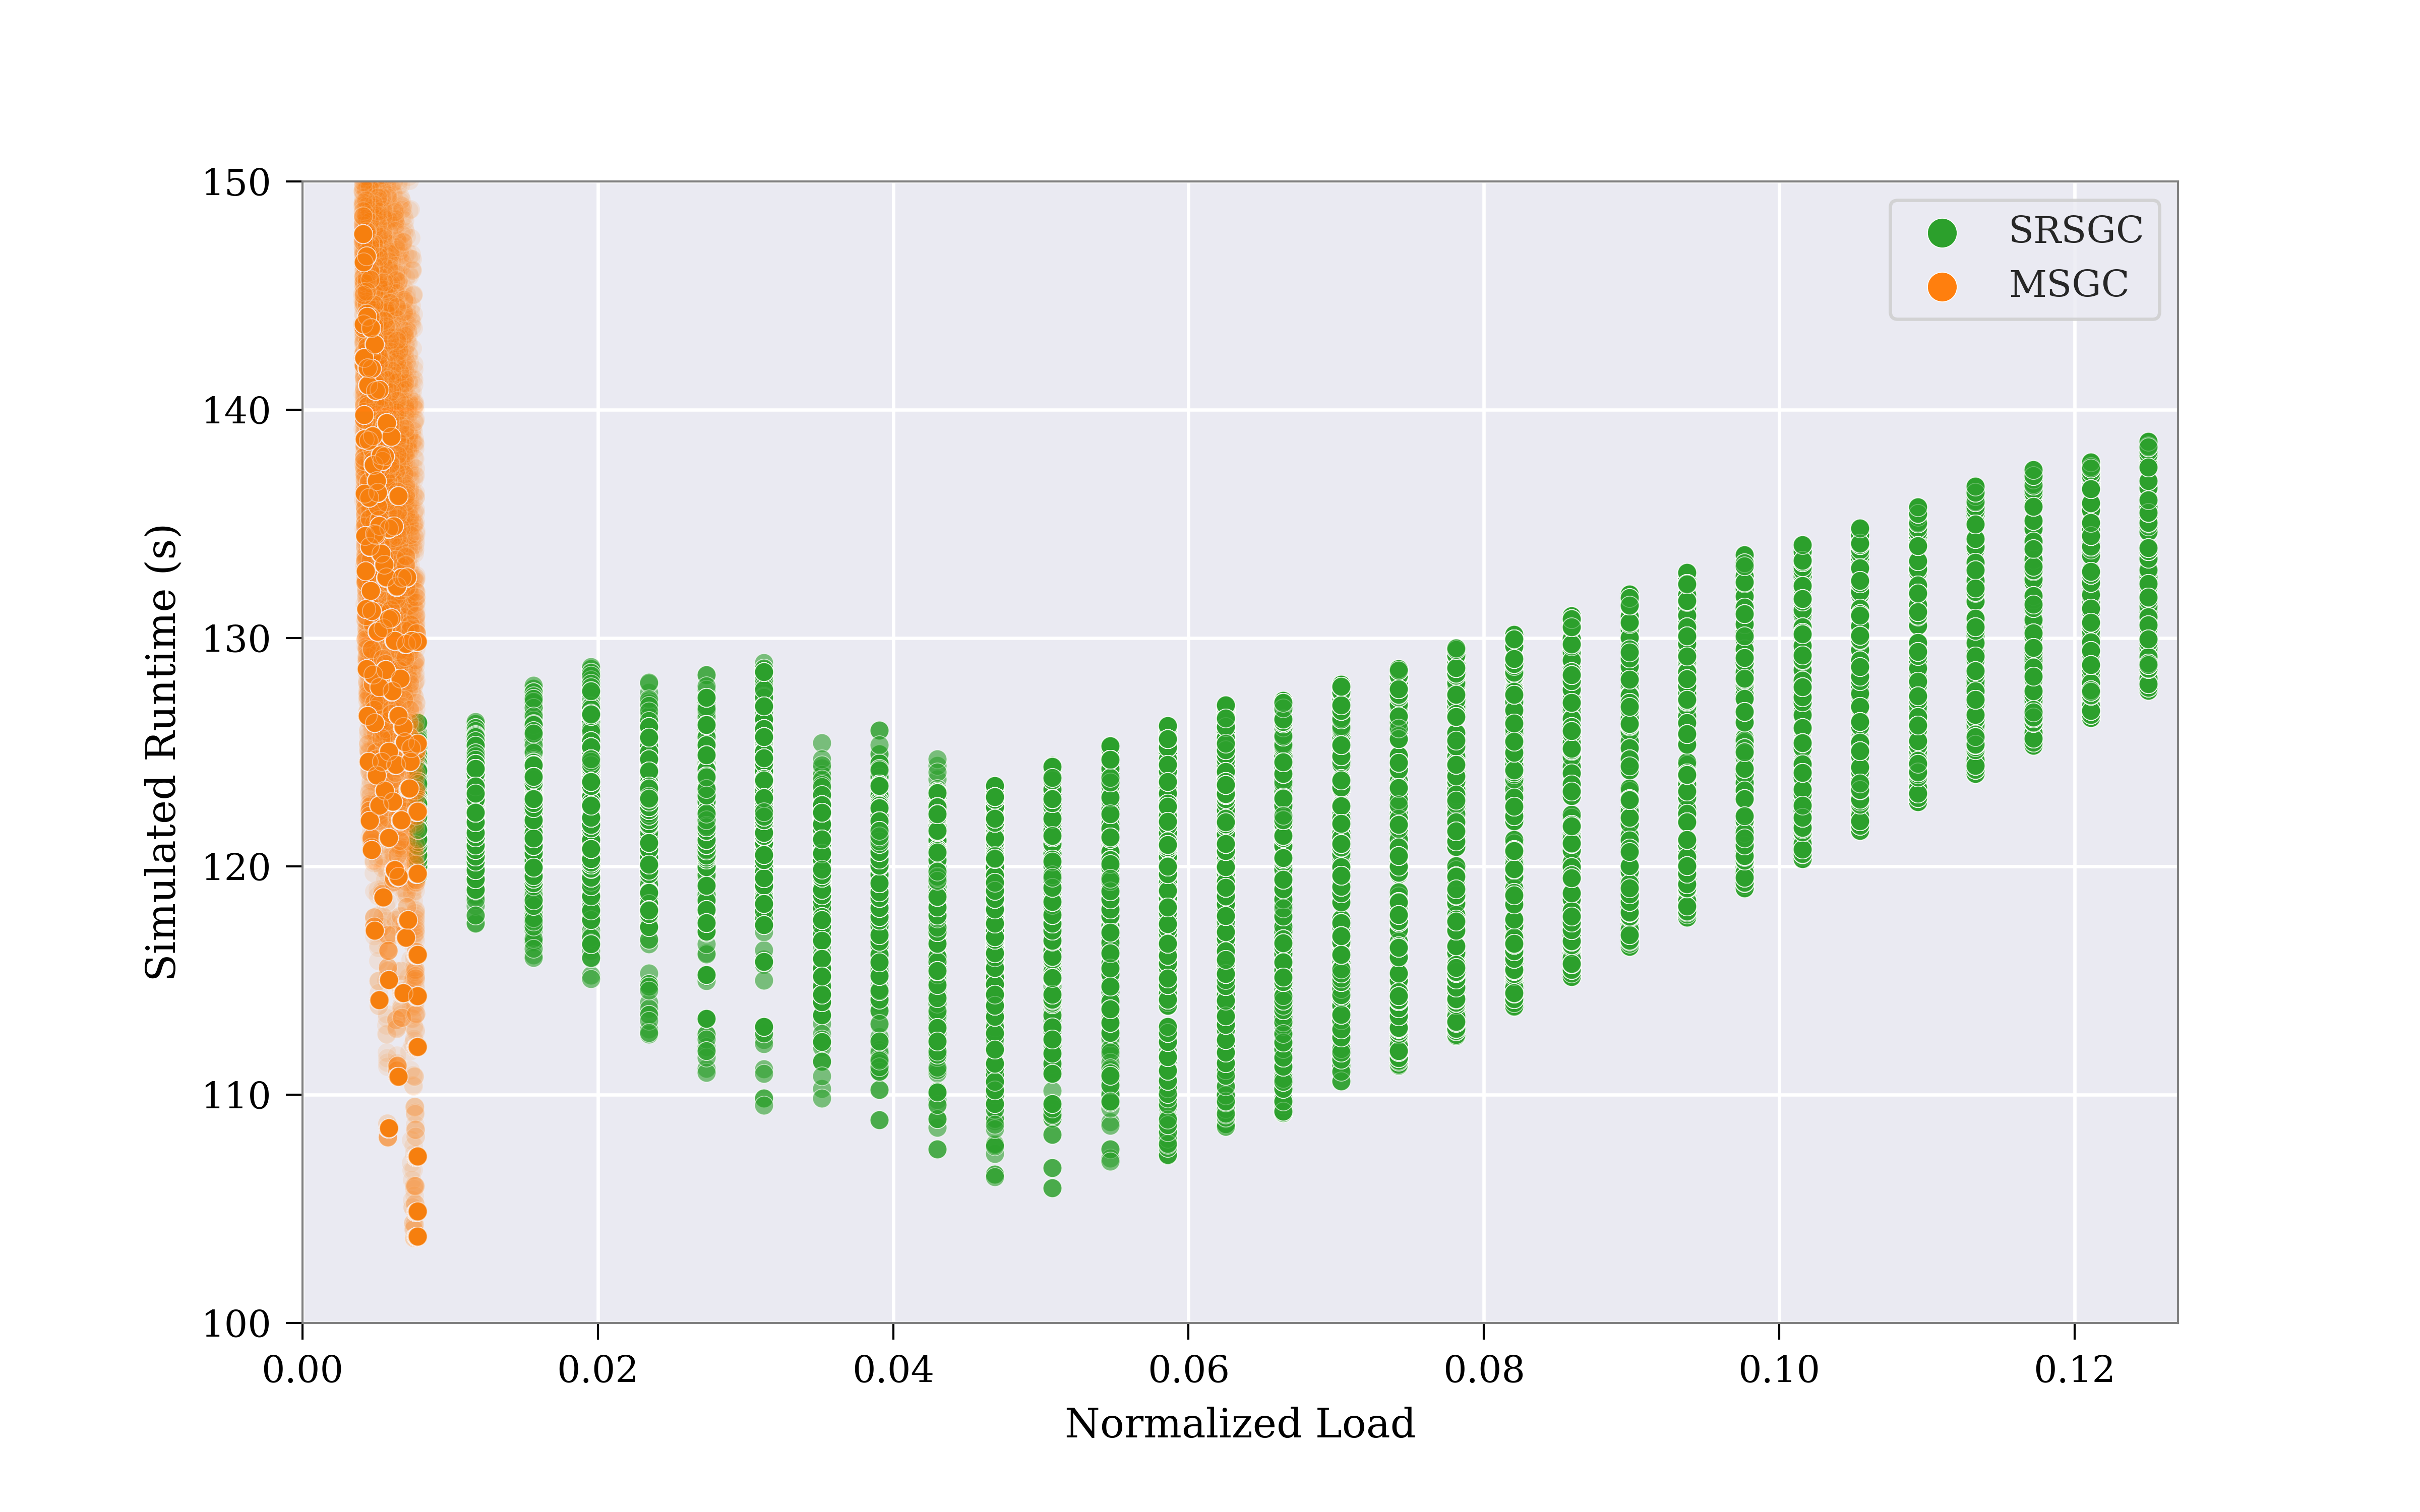
\includegraphics[width=0.65\textwidth]{figures/ch2/6.png}
	\caption{Simulated total run times of calculating 80 jobs using SR-SGC and M-SGC. Each point represents one parameter combination.}
	\label{fig:allparams}
\end{figure}

	For each of the two schemes, we select the parameters corresponding to the smallest total run time. The selected parameters are stated in Table \ref{table:4-1}. Note that as per Remark \ref{rem:comp_load_comparison}, normalized load of M-SGC is upper-bounded by $2/n$, which can also be observed in Fig.~\ref{fig:allparams}.




\section{Problem Definition}

\section{Outcomes}

\section{Future Plans}
